\documentclass[11pt,a4paper]{article}
% CITS4403 report: A4, 11pt, 1-inch margins (rubric). Compile with pdflatex (Overleaf: default settings).
\usepackage[margin=1in]{geometry}
\usepackage[T1]{fontenc}
\usepackage[utf8]{inputenc}
\usepackage{mathptmx}            % Times text and maths
\usepackage{courier}             % scalable typewriter font
\usepackage{amsmath}
\usepackage{graphicx,float,booktabs,tabularx,array}
\usepackage[font=small,labelfont=bf,skip=4pt]{caption}
\usepackage{titlesec}
\usepackage[hidelinks]{hyperref}
\usepackage{url}
\usepackage{microtype}
\usepackage{enumitem}
\usepackage{tikz}
\usepackage{rotating}
\usetikzlibrary{positioning}
\titleformat{\section}{\large\bfseries}{\thesection.}{0.5em}{}
\titleformat{\subsection}{\normalsize\bfseries\itshape}{\thesubsection}{0.5em}{}
\titlespacing*{\section}{0pt}{8pt}{3pt}
\titlespacing*{\subsection}{0pt}{5pt}{2pt}
\linespread{0.95}               % ~12.9pt leading, close to Word's single spacing for 11pt Times
\setlength{\parindent}{0pt}
\setlength{\parskip}{2pt}
\setlength{\abovedisplayskip}{5pt}\setlength{\belowdisplayskip}{5pt}
\setlength{\abovedisplayshortskip}{3pt}\setlength{\belowdisplayshortskip}{4pt}
\setlength{\textfloatsep}{8pt}
\urlstyle{same}

\begin{document}

\begin{center}
{\LARGE\bfseries Chokepoint Disruption in the Global Oil Network\par}
\vspace{2pt}
{\large\itshape A three-layer network-cascade model of the 2026 Strait of Hormuz closure\par}
\vspace{4pt}
{\small Raed Rahmanseresht (21016839) \textperiodcentered{} CITS4403 Computational Modelling \textperiodcentered{} The University of Western Australia\\
October 2026 \textperiodcentered{} Code, data and notebook: \url{https://github.com/raed-ra/cits4403-oil-chokepoint}\par}
\end{center}
\vspace{-4pt}

\section{Background and research questions}

The Strait of Hormuz carried about 20.9\,mb/d of crude oil and petroleum products in 2023, roughly a fifth of world liquids consumption (EIA, 2024). After hostilities began at the end of February 2026, tanker traffic through the strait collapsed: tanker deadweight tonnage fell by about 80\% in the following week (An et al., 2026), and by the second quarter only about 4.9\,mb/d was still flowing (EIA, 2026). Brent crude rose from about \$69/bbl in February to around \$105/bbl in Q2, despite a coordinated IEA release of 400 million barrels on 11 March (IEA, 2026).

The oil system is a complex system (Downey, 2018): a closure's effect is not simply the barrels lost at the strait. Flows reroute until bypass pipelines and canals reach capacity; importing regions compete for the remaining cargoes; prices rise and destroy demand; and shortages pass from oil-intensive sectors such as transport and petrochemicals to the sectors that depend on them. Such cascades are well studied in network science (Motter \& Lai, 2002; Buldyrev et al., 2010), as is the dependence of robustness on topology (Albert, Jeong \& Barabási, 2000).

Among 2026 studies, the closest, An et al. (2026), is a country--sector input--output network in which the blockade directly caps Gulf producers' output; loss reaches 50\% at 32--46\% blockade intensity, but rerouting, price feedback and strategic reserves are not modelled. Devetak, Verschuur and Klimek (2026) simulate ships rerouting around closed chokepoints and find Hormuz losses concentrated in Asian ports, without production, prices or reserves. Sharma and Lau (2026) optimise India's import network under correlated Hormuz and Bab el-Mandeb disruptions, treating the correlation as an assumed probability. Hinz et al. (2026) model trade without explicit rerouting or reserves. None combines physical rerouting through capacitated chokepoints and bypass pipelines with market clearing, location-specific reserves and a production cascade. This project does, and uses the combination to answer six science questions:

\begin{description}[leftmargin=2.2em,labelwidth=1.8em,labelsep=0.4em,itemsep=0pt,topsep=1pt,parsep=0pt,font=\normalfont\bfseries]
\item[Q1] \textbf{Threshold.} As the share of Hormuz flow blocked rises, is there a critical closure level $c^{*}$ at which a localised shortfall becomes systemic production failure?
\item[Q2] \textbf{Interventions.} Which intervention -- bypass capacity, demand restraint or strategic reserve release -- raises $c^{*}$ most, per barrel and at realistic scale?
\item[Q3] \textbf{Correlated closures.} Does closing Bab el-Mandeb as well amplify the damage, and why?
\item[Q4] \textbf{Reserve location.} Does it matter where strategic reserves are held?
\item[Q5] \textbf{Topology or capacity.} Is the real network fragile because of its structure, compared with the random-graph models taught in the unit, or because of its capacities?
\item[Q6] \textbf{Price feedback (extension).} How does $c^{*}$ change when high prices are allowed to cut demand and free oil for other regions?
\end{description}


\section{Originality and contribution}

Like An et al. (2026) and Devetak et al. (2026), this model is a network simulation stepped day by day, whereas Sharma and Lau (2026) solve an optimisation and Hinz et al. (2026) a general equilibrium (Table~\ref{tab:lit}). It is deliberately smaller and simpler -- ten regions rather than countries or ships -- so every delivery can be traced to a rule. Its contribution is therefore not scale or data detail but the coupling: each study models one part of the chain, while this model connects rerouting to the market and to production loss. \textbf{(i) Closure as a network constraint, not a supply cut:} each region's loss emerges from rerouting, bypass capacity and competition between buyers, rather than Gulf exports being removed by assumption. \textbf{(ii) Correlated failure from structure:} the Hormuz--Bab el-Mandeb dependence is physical, not an assumed probability, because the main bypass loads on the Red Sea. \textbf{(iii) Location-specific reserves}, compared with a pooled reserve. \textbf{(iv) Per-barrel and realistic-scale comparison of interventions} on a threshold. \textbf{(v) Taught network models as null models:} Erdős--Rényi, Watts--Strogatz and Barabási--Albert graphs (Erdős \& Rényi, 1959; Watts \& Strogatz, 1998; Barabási \& Albert, 1999) serve as baselines; no lecture case study is reused. \textbf{(vi) Price feedback}, which An et al. (2026) leave to future work.

\begin{table}[t]
\centering\footnotesize
\caption{Scope of this model compared with 2026 studies of the Hormuz closure.}\label{tab:lit}
\renewcommand{\arraystretch}{1.0}\setlength{\tabcolsep}{4pt}
\begin{tabularx}{\textwidth}{@{}>{\raggedright\arraybackslash}p{2.55cm}*{5}{>{\raggedright\arraybackslash}X}@{}}
\toprule
 & \textbf{An et al. (2026)} & \textbf{Devetak et al. (2026)} & \textbf{Sharma \& Lau (2026)} & \textbf{Hinz et al. (2026)} & \textbf{This project} \\ \midrule
\textbf{Model type} & Daily network simulation & Agent-based ship simulation & Stochastic optimisation & General equilibrium & Daily layered network simulation \\
\textbf{Scale} & Countries $\times$ sectors & 35,954 ships, 1,651 ports & 16 nodes (India) & 160 countries, 65 sectors & 10 regions, 37 routes, 5 sectors \\ \midrule
\textbf{How the closure enters} & Cap on Gulf output & Ships rerouted & Scenario arc capacities & Trade barrier on Gulf exports & Limit on one node of a route network \\
\textbf{Rerouting via bypasses} & No & Yes (ship-level) & Yes (optimised) & Elasticities only & Yes (capacitated) \\
\textbf{Production cascade} & Yes (input--output) & No & No & Yes (input bottlenecks) & Yes (five sectors per region) \\
\textbf{Endogenous price} & One-way only & No & No & Yes (equilibrium) & Yes; feedback in extension \\
\textbf{Strategic reserves} & Edge inventories & No & Own national & Excluded & Six regional vs pooled \\
\textbf{Hormuz + Bab el-Mandeb} & No & Not studied & Assumed & No & Emerges from network \\
\textbf{Threshold metric} & Yes (50\% loss) & No & No & No & Yes (10\% loss) \\
\bottomrule
\end{tabularx}
\end{table}


\section{How the model is built}

\subsection{Three layers and how they talk to each other}

The model is three networks stacked on top of each other and run once per simulated day (Figure~\ref{fig:flow}; node and edge counts in Table~\ref{tab:net}). \textbf{Layer~1} is a physical flow network that decides where oil goes. \textbf{Layer~2} is a market network that turns the world shortage into one price and lets each region draw its own strategic reserve. \textbf{Layer~3} is a production network inside each region that turns the oil a region actually receives into lost economic output. In the main model information flows one way. Layer~1 passes each region's unserved demand $u_r$ to Layer~2. Layer~2 subtracts the region's own reserve draw $R_r$ and passes the remaining shortage to Layer~3 as the share of its normal demand $D_r$ that is still supplied,
\begin{equation}\label{eq:link}
x_r = 1-\frac{u_r-R_r}{D_r}, \qquad Q=\sum_r \bigl(D_r-u_r+R_r\bigr),
\end{equation}
while the total oil available $Q$ sets the price. The price does not change demand in Layer~1; that missing arrow is the main simplification, and the extension (Section~\ref{sec:extmodel}) adds it.

\begin{table}[t]
\centering\footnotesize
\caption{The nodes and edges of each layer.}\label{tab:net}
\renewcommand{\arraystretch}{1.0}\setlength{\tabcolsep}{4pt}
\begin{tabularx}{\textwidth}{@{}>{\raggedright\arraybackslash}p{2.3cm}>{\raggedright\arraybackslash}X>{\raggedright\arraybackslash}X>{\raggedright\arraybackslash}p{2.5cm}@{}}
\toprule
\textbf{Layer} & \textbf{Nodes} & \textbf{Edges} & \textbf{Passes on} \\ \midrule
\textbf{1 Routing} & 10 consumer regions; 11 producer nodes (6 export); 8 chokepoints; 2 bypass pipelines & 37 directed routes producer $\rightarrow$ chokepoint(s) $\rightarrow$ consumer, each with a voyage time (Middle East 17, North America 6, Africa 5, Latin America 4, CIS 3, East Siberia 2; 9 via pipelines) & Unserved demand $u_r$ \\
\textbf{1 as a graph (Q5)} & 22: 6 exporters, 8 chokepoints, 8 importing regions & 39 undirected edges & Betweenness, max-flow \\
\textbf{2 Market} & 1 world price, 10 regions, 6 reserves & 10 region--price edges (elasticity $e_r$); 6 reserve $\rightarrow$ own-region edges & Price $p$; oil share $x_r$ \\
\textbf{3 Production} (in each of 10 regions) & 5 sectors + 1 oil input & 5 oil $\rightarrow$ sector edges ($\delta_s$); 8 supplier $\rightarrow$ user edges ($a_{js}$) & Loss $L_r$; threshold $c^{*}$ \\
\bottomrule
\end{tabularx}
\end{table}

\subsection{Layer 1: routing network}

Ten regions each have a producer node and a consumer node, with East Siberia as an export-only node (Figures~\ref{fig:map}--\ref{fig:mapq2}). Production (EIA, 2025 data) and consumption (Energy Institute, 2024 data) are on a total-liquids basis, and chokepoints carry EIA (2024) normal flows. Open straits have no capacity limit; engineered passages do (Suez+SUMED 10.0\,mb/d, Panama 3.5\,mb/d), as do the Saudi East-West pipeline (7.0\,mb/d) and the UAE's ADCOP line to Fujairah (1.5\,mb/d), each a single daily budget shared by every route that uses it. A closure fraction $c$ limits a passage to $(1-c)F^{0}$, where $F^{0}$ is its normal flow (20.9\,mb/d for Hormuz). All numbers and sources are in \texttt{data/DATA\_AND\_SOURCES.md}.

Each day oil is allocated from scratch. A region first meets its demand $D_r$ from its own production $P_r$, $d_r=\min(P_r,D_r)$, so domestic oil can never be bid away. Exports are split into contracted and spot cargoes by a spot share $\kappa_r$. Stage~1 sends contracted cargoes by the fastest routes; every transfer sends the minimum of the buyer's remaining need, the producer's remaining oil, the room left at each chokepoint on the route, the tanker capacity left (fleet $=$ world supply $\times$ 20 days $\times$ 1.25) and any route or pipeline limit. When a route fills, oil spills onto the next fastest -- the congestion cascade. In Stage~2, spot cargoes go to the buyer with the highest netback $n_{rk}$ (region $r$ buying via route $k$),
\begin{equation}\label{eq:bid}
\pi_r = 1 + 4\left(\frac{s_r}{D_r}\right)^{2}, \qquad n_{rk} = \pi_r - 0.01\,\tau_k ,
\end{equation}
where $\pi_r$ is region $r$'s scarcity premium, $s_r$ its shortfall after Stage~1 and $\tau_k$ the voyage time of route $k$ in days; freight is small relative to scarcity, so the most desperate buyer is served first. A \emph{complexity uplift} gives complex refineries up to 15\% more product per barrel (Nelson index), a proxy for crude-grade matching. The output is each region's unserved demand $u_r$.

\subsection{Layer 2: market and reserves}

The world price index $p$ ($p=1$ is \$69/bbl) clears constant-elasticity demand against the oil available,
\begin{equation}\label{eq:price}
\sum_{r} D_r\, p^{\,e_r} = Q, \qquad \text{Brent} = \$69 \times p ,
\end{equation}
solved by bisection, with short-run elasticities $e_r$ (the \% change in demand per 1\% change in price) from $-0.05$ (North America; Ghouri, 2001) to $-0.25$ (Africa), within the range of Cooper (2003); over time the price moves 12\% of the way to the clearing value each day. Strategic reserves (China 1,400\,Mb, Japan/Korea 449, United States 285, Europe 179, Other Asia 50, India 39) each draw $R_r=\min(u_r,\ \text{maximum rate},\ \text{stock left})$ and cover only their own region, because a national reserve cannot be redirected to another country's shortage.

\subsection{Layer 3: production cascade}

Within each region, five sectors with weights $w_s$ equal to their shares of oil use (transport 0.57, petrochemicals 0.21, agriculture/residential 0.11, industry 0.07, power 0.04; OPEC, 2024) depend on oil with intensity $\delta_s$ and on each other, $a_{js}$ being how much sector $s$ needs supplier sector $j$ (Figure~\ref{fig:layers}). Given $x$ from Equation~\eqref{eq:link}, each sector's output $y_s$ is
\begin{equation}\label{eq:cascade}
\begin{aligned}
\text{direct}_s &= 1-\delta_s(1-x), & \text{upstream}_s &= 1-\textstyle\sum_j a_{js}\,(1-y_j),\\
y_s &= z_s\, g(z_s), \quad z_s=\min(\text{direct}_s,\text{upstream}_s), & g(z) &= \bigl[1+e^{-(z-0.45)/0.06}\bigr]^{-1},
\end{aligned}
\end{equation}
where $z_s$ is the more limiting of the two and $g$ is a logistic gate whose \emph{centre} (0.45) is the input share at which it is half shut: well below it a sector cannot operate at all. Equation~\eqref{eq:cascade} is iterated to a fixed point, so a supplier's failure reaches its users. A region's systemic loss and the critical blockade intensity are
\begin{equation}\label{eq:loss}
L_r = \sum_s w_s\,(1-y_s), \qquad c^{*} = \min\Bigl\{\,c \;:\; \max_r L_r(c) > 0.10 \Bigr\}.
\end{equation}

\subsection{Extension: closing the loop from price to demand}\label{sec:extmodel}

The extension (\texttt{experiment\_feedback.py}) adds the missing arrow from Layer~2 back to Layer~1. Each day $t$ every region cuts demand in response to the price, by at most 20\%:
\begin{equation}\label{eq:ext}
\text{cut}_r(t) = D_r\,\min\bigl(1-p(t)^{\,e_r},\ 0.20\bigr), \qquad D_r(t+1) = D_r-\text{cut}_r(t), \qquad x_r = 1-\frac{\text{cut}_r+u_r}{D_r}.
\end{equation}
The oil a region stops buying re-enters the routing, where other regions can buy it; the price moves 12\% a day towards the level at which capped demand equals the oil physically available; and because a price-driven cut is still oil a sector does not receive, it counts as lost input in Layer~3. The cap reflects that short-run demand cannot fall without limit.

\subsection{Assumptions and justification}

The 10\% criterion marks the onset of systemic damage rather than collapse (An et al. use 50\%), since the policy aim is to avoid entering the failure regime. Allocation is a single greedy pass, not an equilibrium, which keeps every delivery traceable to a rule but concentrates trade on short routes; all liquids are interchangeable. Spot shares, most sector dependencies, the gate and several elasticities are assumptions, tested in Section~\ref{sec:q1}. Every run starts from normal conditions; routing reaches steady state on day one, so time matters only for reserves, prices and time-varying closures.


\section{Experimental design}

Each experiment answers one question. Outcomes are unserved demand (mb/d), worst-region loss $\max_r L_r$, Brent (\$/bbl) and $c^{*}$, found by bisection (repeatedly halving the closure interval, 12 times). Runs last 150 days (400 for reserves); the model is deterministic, so one run per setting suffices except for random graphs. \textbf{Q1:} Hormuz closure is swept from 0 to 100\% in 5\% steps and $c^{*}$ computed; robustness is tested by moving the gate centre from 30\% to 60\%, removing the complexity uplift, and comparing four 150-day closure schedules between 30\% and 80\% (sudden then easing, the reverse, a linear ramp, a 15-day oscillation) with equal blockade-days (the sum of daily closure fractions). \textbf{Q2:} at equal size ($\sim$3\,mb/d) the cases are +3\,mb/d of Saudi pipeline capacity, a 2.9\% demand cut in every region, and every reserve draw rate scaled by 3/11; at realistic size, +2\,mb/d, a 3\% cut, full draw rates ($\sim$11\,mb/d), and all three combined; $c^{*}$ is recomputed for each and the reserve case followed for 400 days at 71\% closure. \textbf{Q3:} the Q1 sweep is repeated with Bab el-Mandeb fully closed. \textbf{Q4:} at full closure, Brent is tracked with no reserves, regional reserves, and a hypothetical pooled reserve drawing at the same total rate. \textbf{Q5:} on the 22-node graph, betweenness (the share of shortest paths through a node) is computed and the most central chokepoint removed; the lost flow capacity (producer-to-consumer maximum flow, unit edge capacities) is compared with 200 Erdős--Rényi, Watts--Strogatz ($p=0.1$), Barabási--Albert and degree-preserving rewired graphs (edges shuffled, each node's degree kept) of equal size. \textbf{Q6:} the Q1 sweep and $c^{*}$ are repeated with the extension, with caps of 10, 20 and 30\%. \textbf{Validation:} at the observed Q2 2026 closure (23\% open), emergent corridor flows and the price are compared with EIA data; Hormuz flow itself is set from observation and is not a test.


\section{Results}

\subsection{Q1: the critical threshold}\label{sec:q1}

As Hormuz closes (Figure~\ref{fig:closure}), the Saudi pipeline fills and Bab el-Mandeb flow rises to the pipeline's 7.0\,mb/d limit by 40\% closure. Unserved demand stays near zero until about 45\% closure and then rises almost linearly, to 6.6\,mb/d at 70\% and 12.8\,mb/d at full closure. The critical blockade intensity is $c^{*}=$\,\textbf{53.1\%}. The damage is concentrated: at full closure Other Asia loses 67\% of its demand and China 37\%, while Europe, India and North America remain fully supplied, and any region given half its oil loses 55\% of its output. $c^{*}$ stays within 52.6--53.1\% as the gate centre moves from 30\% to 60\% and falls to 51\% without the complexity uplift. At matched exposure, a 15-day oscillation causes 31\% more average unserved demand than a smooth ramp (4.26 against 3.26\,mb/d), while reversing the order of a sudden closure changes nothing.

\subsection{Q2: interventions}

Figure~\ref{fig:interv} shows the rise in $c^{*}$. At equal size, bypass capacity raises it by 14.4 percentage points, demand restraint by 6.5 and reserves by 5.1. At realistic size reserves give the largest gain (+18.6), ahead of bypass (+9.6) and restraint (+6.8); all three together add 38.0 points, to about 91\%. The reserve gain is temporary: at 71\% closure the worst region stays below 10\% loss only until China's reserve runs out on day 350, and becomes systemic the next day.

\subsection{Q3: correlated closures}

Closing Bab el-Mandeb as well as 70\% of Hormuz raises unserved demand from 6.6 to 9.9\,mb/d (+49\%), and damage begins at about 25\% Hormuz closure instead of 45\% (Figure~\ref{fig:closure}, right). Closed alone, Bab el-Mandeb has almost no effect.

\subsection{Q4: reserve location}

At full closure, on day 100 Brent is about \$236/bbl with no reserves, \$151 with regional reserves and \$81 with a pooled reserve of the same draw rate (Figure~\ref{fig:reserves}). The United States, Europe and India are not short, so about 500\,Mb is never drawn, while China exhausts its 1,400\,Mb on day 350.

\subsection{Q5: topology or capacity}

Betweenness ranks Malacca (0.31) and the Cape (0.30) highest and Hormuz almost last (0.03), because Hormuz serves one origin that has other exits (Figure~\ref{fig:topo}). Removing the most central chokepoint disconnects no producer--consumer pair and costs 5.6\% of flow capacity, against mean losses of 12\% (Erdős--Rényi), 14\% (Barabási--Albert), 15\% (rewired) and 24\% (Watts--Strogatz) for random graphs of equal size.

\subsection{Q6: price feedback}

With the extension, $c^{*}$ rises from 53\% to 64\% and the worst region's loss at full closure falls from 89\% to 23\%: at about \$259/bbl every region cuts back, instead of Asia absorbing the shortage (Figure~\ref{fig:ext}). This takes about a month; at 60\% closure the worst region loses 18.6\% on day 1 but 8.3\% by day 30. It is robust to the cap (63.9\% at 20 or 30\%; 69.1\% at 10\%).

\textbf{Validation.} At the Q2 2026 closure the model gets the direction of rerouting right but under-predicts its size (Bab el-Mandeb 7.0 against 8.1\,mb/d observed, Suez+SUMED 3.6 against 5.8, Malacca 9.9 against 16.6). The price is \$94/bbl with full regional reserves and \$143/bbl with none; the observed $\sim$\$105 lies inside this bracket.


\section{Discussion and conclusions}

\textbf{Q1.} There is a sharp transition at about 53\% closure, produced by three interacting non-linearities: bypass capacity absorbs the first $\sim$45\% of a closure and then saturates; netback bidding concentrates the remaining shortfall on the regions with the least alternative supply; and the production cascade amplifies a loss once supplier sectors fail. It exceeds the 32--46\% of An et al. (2026) despite a stricter criterion (10\% against 50\%) because rerouting absorbs much of the early shock when a closure constrains a network rather than capping Gulf output. Convexity -- damage rising faster than closure -- makes a swinging disruption worse than a steady one. \textbf{Q2.} Per barrel, bypass capacity is most effective because it releases stranded Gulf supply that can travel to wherever the shortage is; restraint is spread over regions that are not short, and reserves stay where they are held. At realistic scale reserves help most, but only while they last: reserves buy time, bypass buys resilience. \textbf{Q3.} The Saudi bypass exits through the Red Sea, so the larger the bypass, the more the system depends on Bab el-Mandeb: the safety valve and the vulnerability are the same route, and unlike India's diversified network in Sharma and Lau (2026) this risk cannot be diversified away. \textbf{Q4.} The constraint on reserves is not how much oil exists but whether it sits where the shortage falls; pooling would roughly halve the price. \textbf{Q5.} By connectivity or betweenness Hormuz looks unimportant; its importance lies in the volume it carries, and the network's parallel routes make it more robust than any random baseline: vulnerability comes from capacity concentration, not structure, which is why a flow model was needed. \textbf{Q6.} Letting prices spread the shortage raises the threshold, so 53\% is best read as the threshold for a closure's first weeks and 64\% as the threshold once markets adjust.

These conclusions hold within clear limits. Allocation is a greedy single pass, not an equilibrium, and in the main model price does not feed back into routing, so damage in Asia is probably overstated; the extension shows by how much. Refined products and crude grades are not modelled, which explains much of the under-prediction of corridor flows. The threshold is insensitive to the assumed parameters but moved between 38\% and 56\% across structural revisions during development, so it is this model's estimate rather than a property of the world. Future work: bilateral trade data, an equilibrium allocation, a refined-products layer and an input--output cascade (An et al., 2026).

In conclusion, a Hormuz closure turns systemic near half closure, and moving stranded Gulf oil helps most.


\section*{References}
\begin{list}{}{\leftmargin=1.5em\itemindent=-1.5em\itemsep=1pt\parsep=0pt}\small

\item Albert, R., Jeong, H. \& Barabási, A.-L. (2000). Error and attack tolerance of complex networks. \emph{Nature}, 406, 378--382.

\item An, F., Ren, S., Liu, X., Liu, S. \& Cui, J. (2026). A network-cascade framework for short-run production failure under maritime-energy chokepoint disruption. \emph{Mathematics}, 14(10), 1708. \url{https://doi.org/10.3390/math14101708}

\item Barabási, A.-L. \& Albert, R. (1999). Emergence of scaling in random networks. \emph{Science}, 286, 509--512.

\item Buldyrev, S.V., Parshani, R., Paul, G., Stanley, H.E. \& Havlin, S. (2010). Catastrophic cascade of failures in interdependent networks. \emph{Nature}, 464, 1025--1028.

\item Cooper, J.C.B. (2003). Price elasticity of demand for crude oil: estimates for 23 countries. \emph{OPEC Review}, 27(1), 1--8.

\item Devetak, M., Verschuur, J. \& Klimek, P. (2026). Adaptive rerouting reshapes impacts of maritime chokepoint disruptions. arXiv:2606.13431.

\item Downey, A.B. (2018). \emph{Think Complexity: Complexity Science and Computational Modeling} (2nd ed.). O'Reilly.

\item EIA (2024). \emph{World Oil Transit Chokepoints}. U.S. Energy Information Administration. \url{https://www.eia.gov/}

\item EIA (2026). \emph{Short-Term Energy Outlook} and \emph{International Energy Statistics}. U.S. Energy Information Administration. \url{https://www.eia.gov/outlooks/steo/}

\item Energy Institute (2024). \emph{Statistical Review of World Energy}. \url{https://www.energyinst.org/statistical-review}

\item Erdős, P. \& Rényi, A. (1959). On random graphs I. \emph{Publicationes Mathematicae}, 6, 290--297.

\item Ghouri, S.S. (2001). Oil demand in North America: 1980--2020. \emph{OPEC Review}, 25(4), 339--355.

\item Hinz, J., Mahlkow, H., Sogalla, R. \& Willmann, G. (2026). \emph{The Cost of Closing the Strait of Hormuz: Energy Bottlenecks and Global Food Security}. Kiel Policy Brief 206. Kiel Institute for the World Economy.

\item IEA (2026). \emph{Strait of Hormuz} and coordinated emergency stock release of 11 March 2026. International Energy Agency. \url{https://www.iea.org/about/oil-security-and-emergency-response/strait-of-hormuz}


\item Motter, A.E. \& Lai, Y.-C. (2002). Cascade-based attacks on complex networks. \emph{Physical Review E}, 66, 065102.

\item OPEC (2024). \emph{World Oil Outlook 2024}. Organization of the Petroleum Exporting Countries.

\item Sharma, M. \& Lau, H.C. (2026). Securing the flow: maritime energy resilience under correlated and decision-dependent disruptions. arXiv:2605.11990.


\item Watts, D.J. \& Strogatz, S.H. (1998). Collective dynamics of `small-world' networks. \emph{Nature}, 393, 440--442.

\end{list}


\clearpage
\section*{Figures}

\begin{figure}[H]
\centering
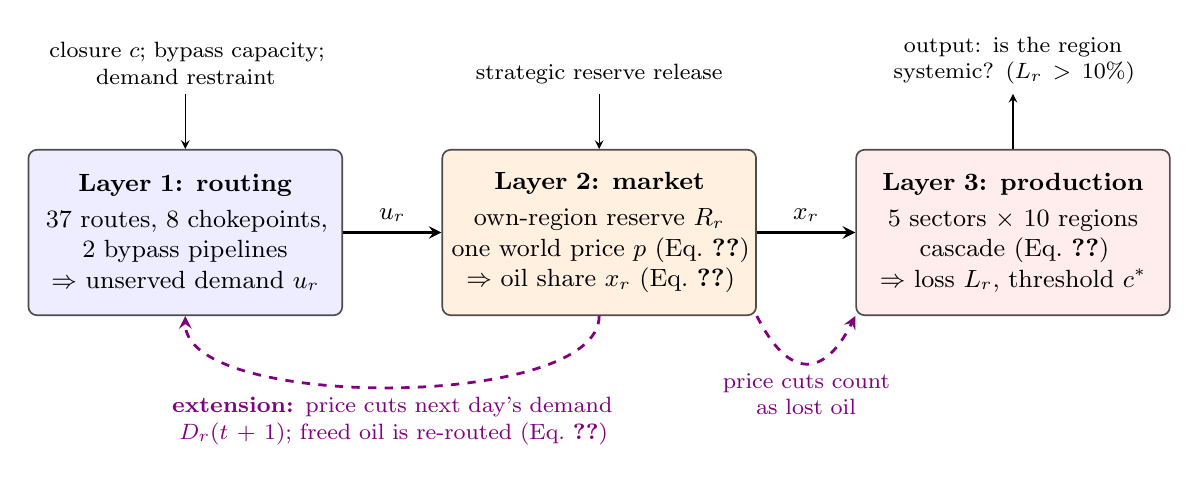
\begin{tikzpicture}[font=\small,>=stealth,
  box/.style={draw=black!70,rounded corners=3pt,align=center,text width=3.75cm,minimum height=2.1cm,line width=0.6pt},
  inp/.style={align=center,font=\footnotesize,text width=3.75cm}]
\node[box,fill=blue!7] (L1) {\textbf{Layer 1: routing}\\[2pt] 37 routes, 8 chokepoints,\\ 2 bypass pipelines\\ $\Rightarrow$ unserved demand $u_r$};
\node[box,fill=orange!12,right=1.25cm of L1] (L2) {\textbf{Layer 2: market}\\[2pt] own-region reserve $R_r$\\ one world price $p$ (Eq.~\ref{eq:price})\\ $\Rightarrow$ oil share $x_r$ (Eq.~\ref{eq:link})};
\node[box,fill=red!7,right=1.25cm of L2] (L3) {\textbf{Layer 3: production}\\[2pt] 5 sectors $\times$ 10 regions\\ cascade (Eq.~\ref{eq:cascade})\\ $\Rightarrow$ loss $L_r$, threshold $c^{*}$};
\draw[->,line width=1pt] (L1) -- node[above]{$u_r$} (L2);
\draw[->,line width=1pt] (L2) -- node[above]{$x_r$} (L3);
\node[inp,above=0.7cm of L1] (i1) {closure $c$; bypass capacity;\\ demand restraint};
\node[inp,above=0.7cm of L2] (i2) {strategic reserve release};
\node[inp,above=0.7cm of L3] (i3) {output: is the region systemic? ($L_r>10\%$)};
\draw[->] (i1) -- (L1); \draw[->] (i2) -- (L2); \draw[<-] (i3) -- (L3);
\draw[->,dashed,line width=1pt,violet] (L2.south) .. controls +(0,-1.2) and +(0,-1.2) .. node[below,font=\footnotesize,text width=7cm,align=center]{\textbf{extension:} price cuts next day's demand $D_r(t+1)$; freed oil is re-routed (Eq.~\ref{eq:ext})} (L1.south);
\draw[->,dashed,line width=1pt,violet] (L2.south east) .. controls +(0.4,-0.8) and +(-0.4,-0.8) .. node[below,font=\footnotesize,text width=3.2cm,align=center]{price cuts count as lost oil} (L3.south west);
\end{tikzpicture}
\caption{How the three layers exchange information each simulated day. Solid arrows: the main model, in which information flows one way. Dashed arrows: the extension, which closes the loop from price back to demand. Interventions enter where they act: bypass and restraint in Layer~1, reserves in Layer~2.}\label{fig:flow}
\end{figure}


\begin{sidewaysfigure}
\centering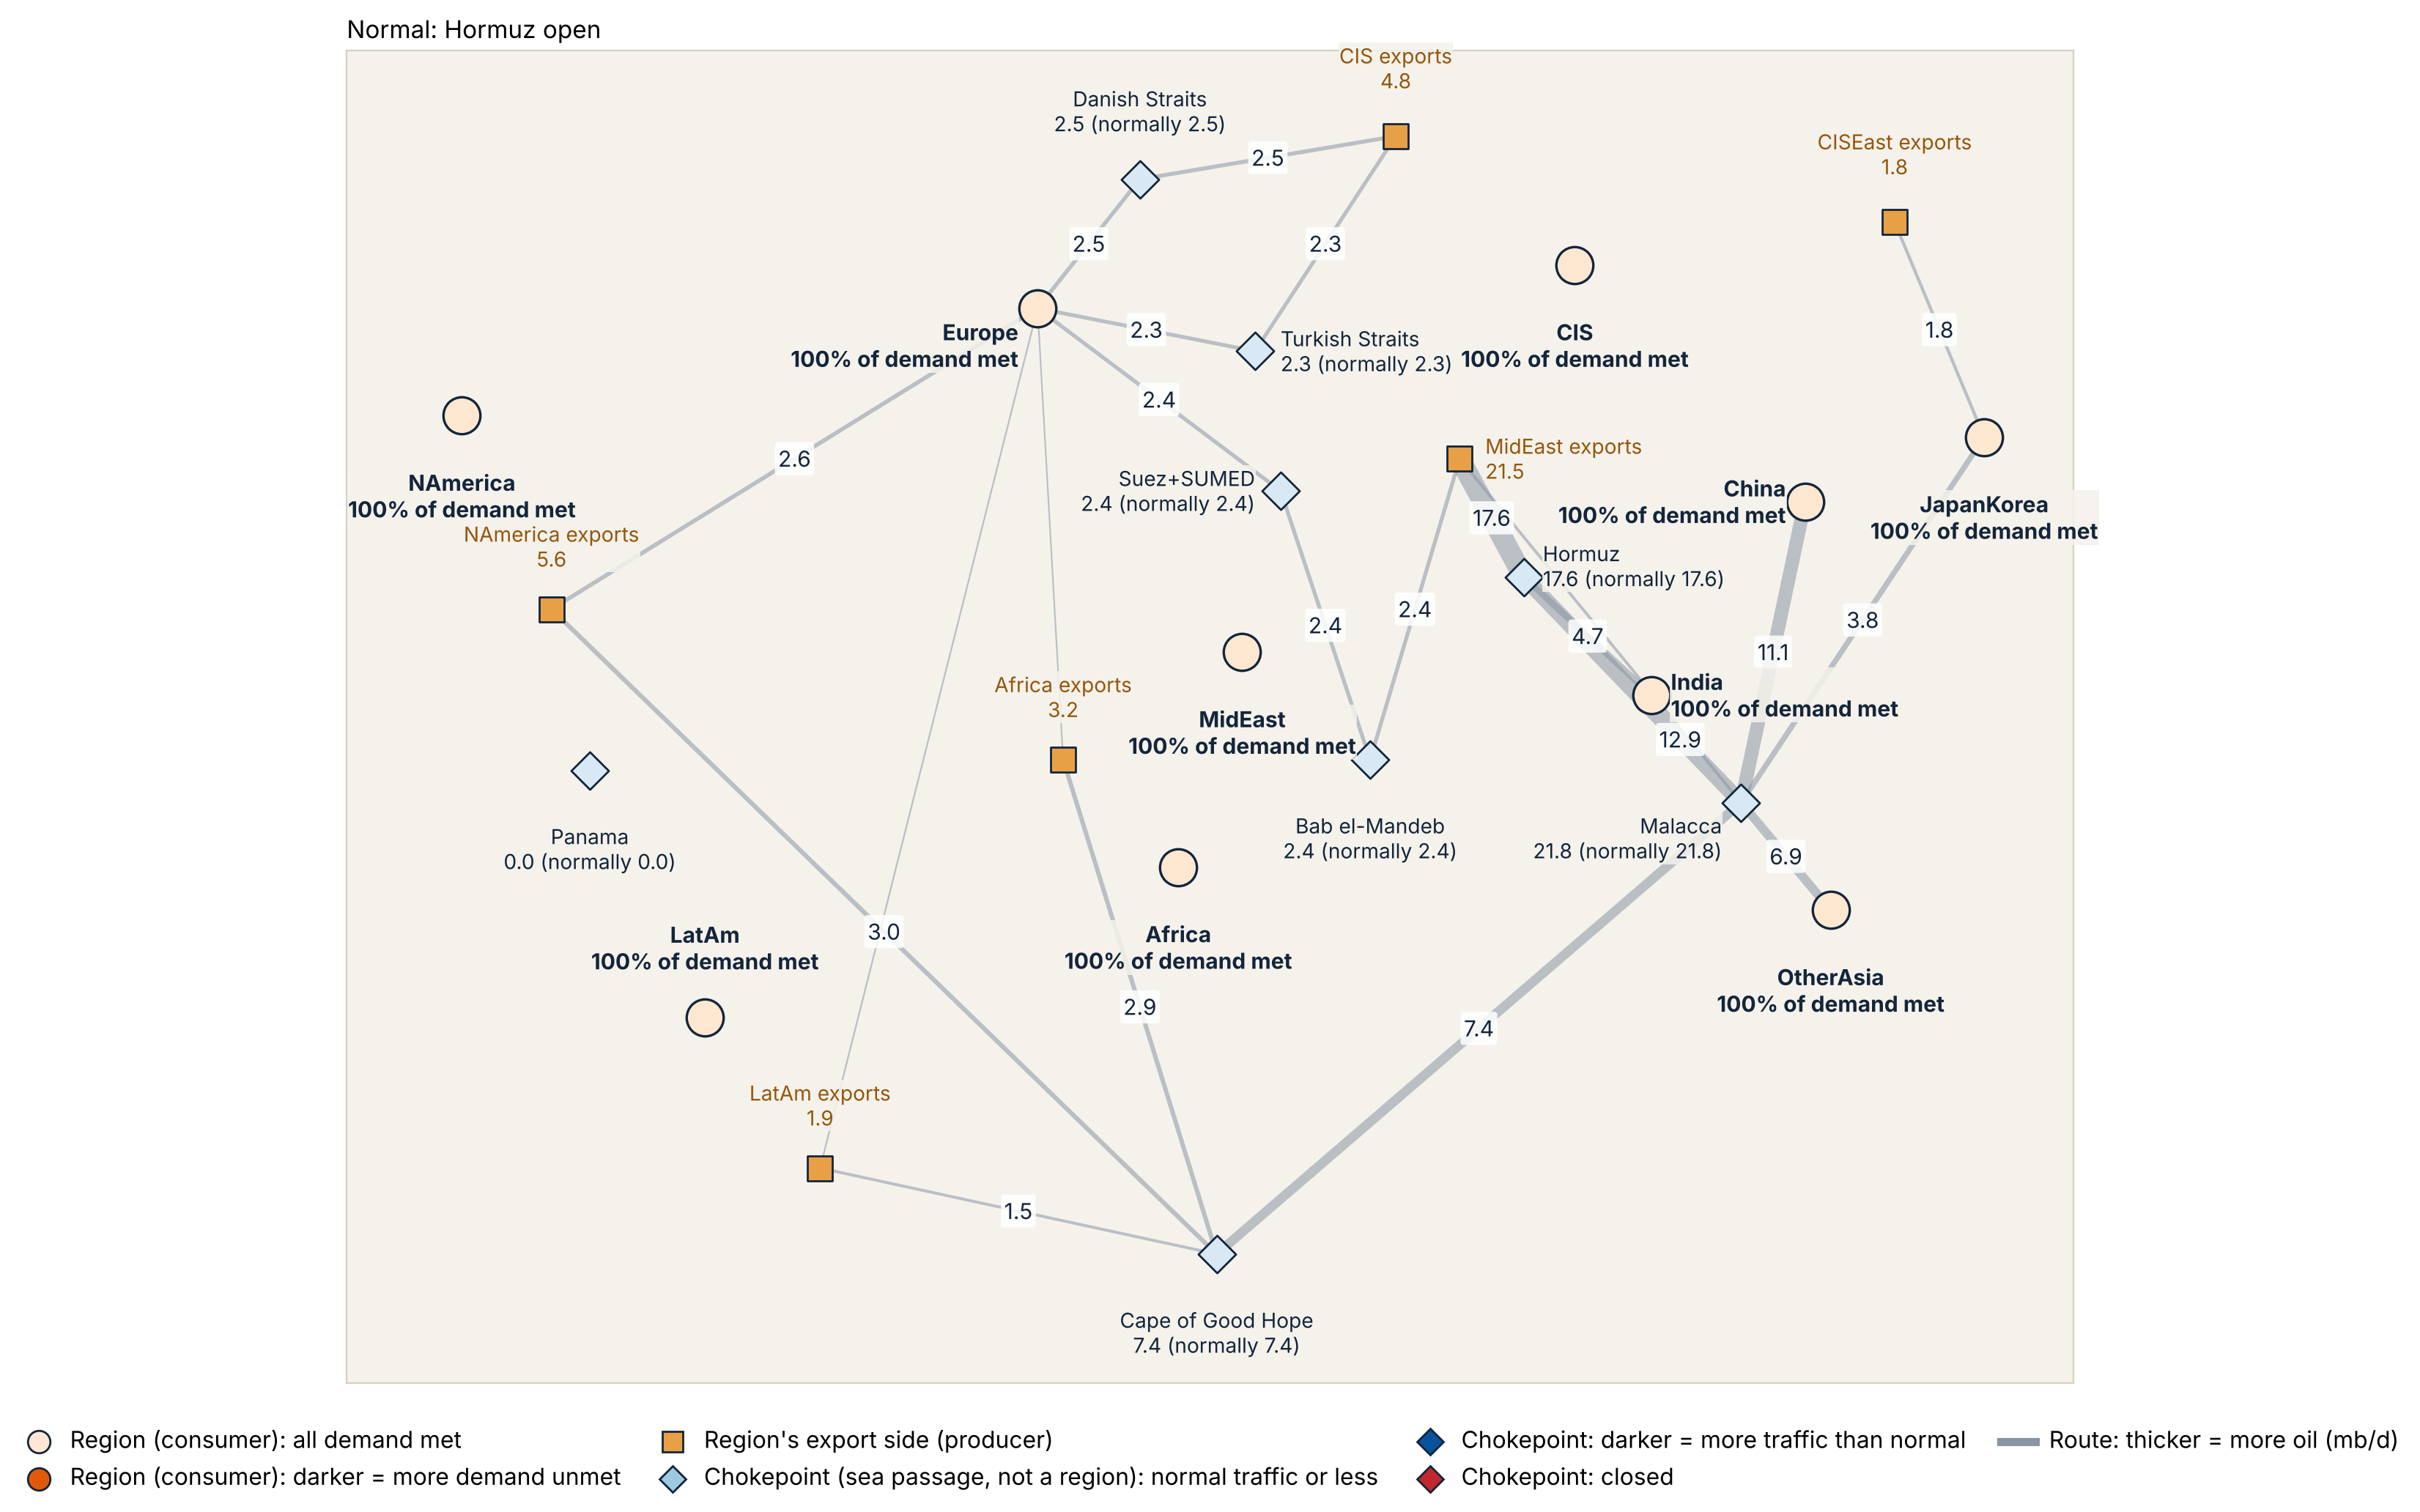
\includegraphics[width=0.97\textheight]{figures/map_normal.png}
\caption{The route network under normal conditions (Hormuz open). Squares are regions' export (producer) nodes, circles consumer nodes shaded by unmet demand, diamonds chokepoints shaded by traffic relative to normal; line width and numbers are flow (mb/d).}\label{fig:map}
\end{sidewaysfigure}

\begin{sidewaysfigure}
\centering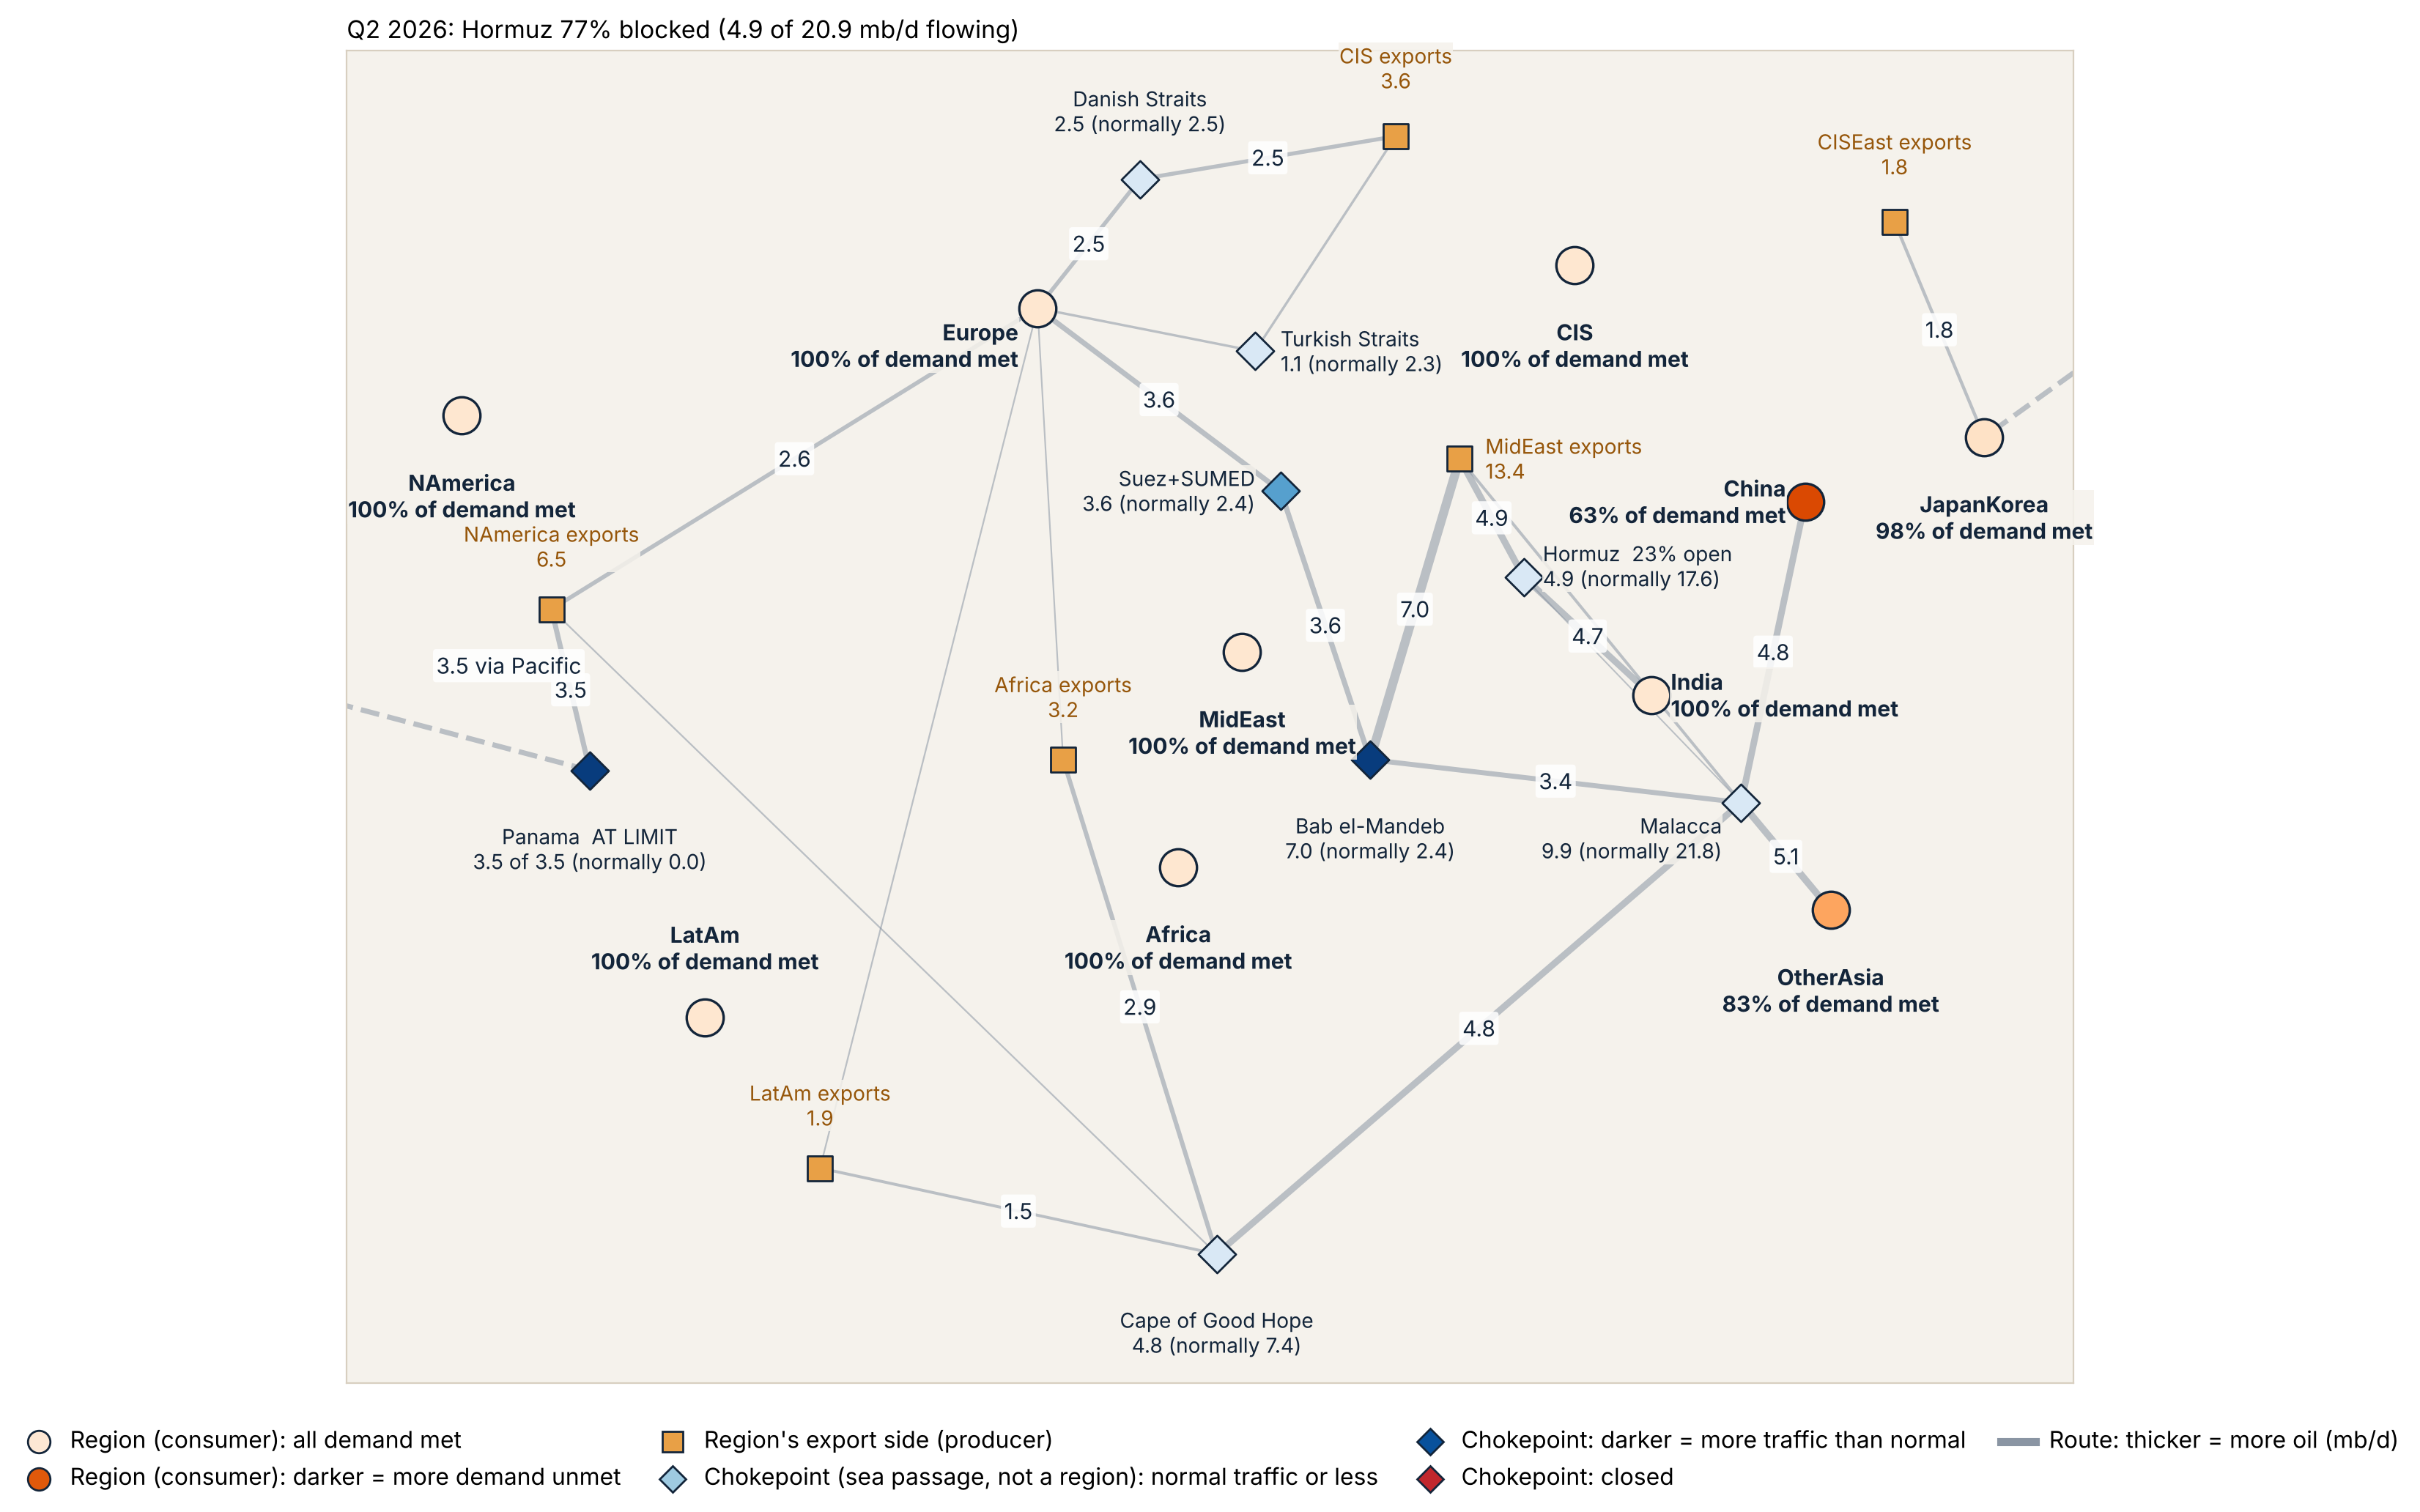
\includegraphics[width=0.97\textheight]{figures/map_q2.png}
\caption{The same network at the observed Q2 2026 closure (Hormuz 77\% blocked): the Saudi pipeline fills and carries 7.0\,mb/d out through Bab el-Mandeb, North American oil crosses the Pacific through Panama, and China falls to 63\% of demand met.}\label{fig:mapq2}
\end{sidewaysfigure}

\begin{figure}[H]
\centering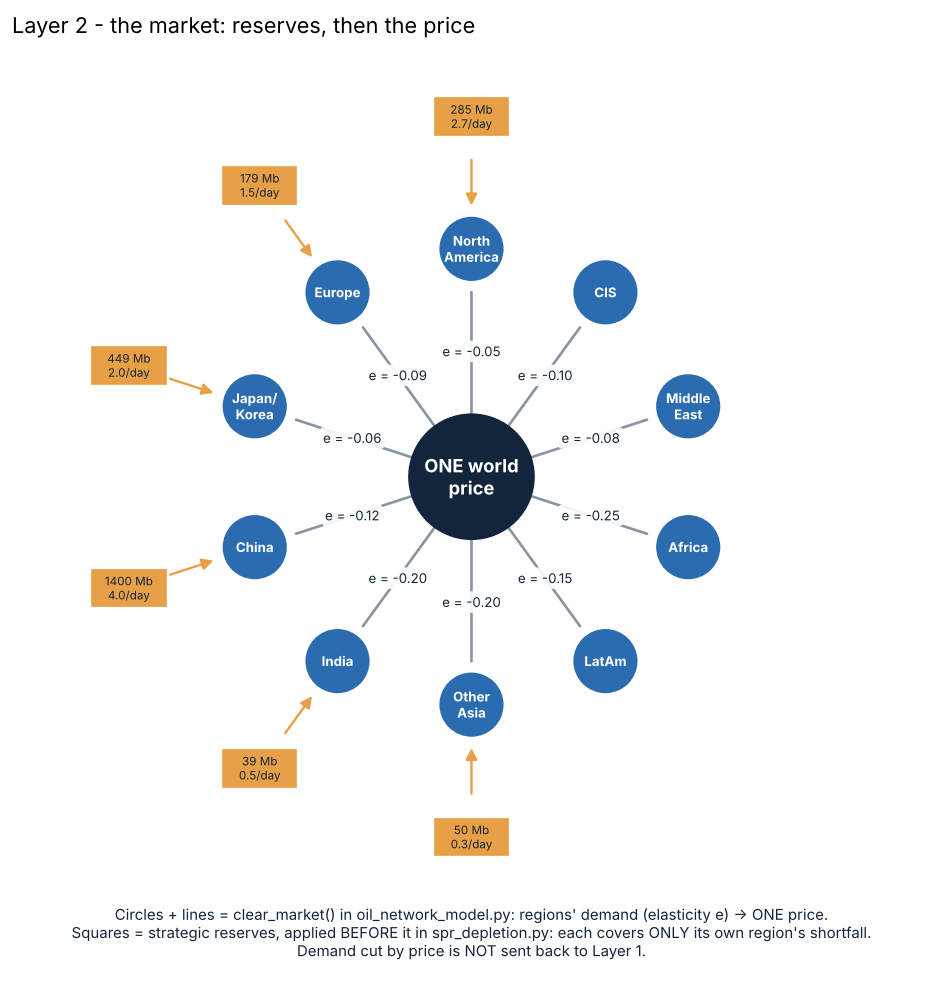
\includegraphics[width=0.49\textwidth]{figures/layer2_market.png}\hfill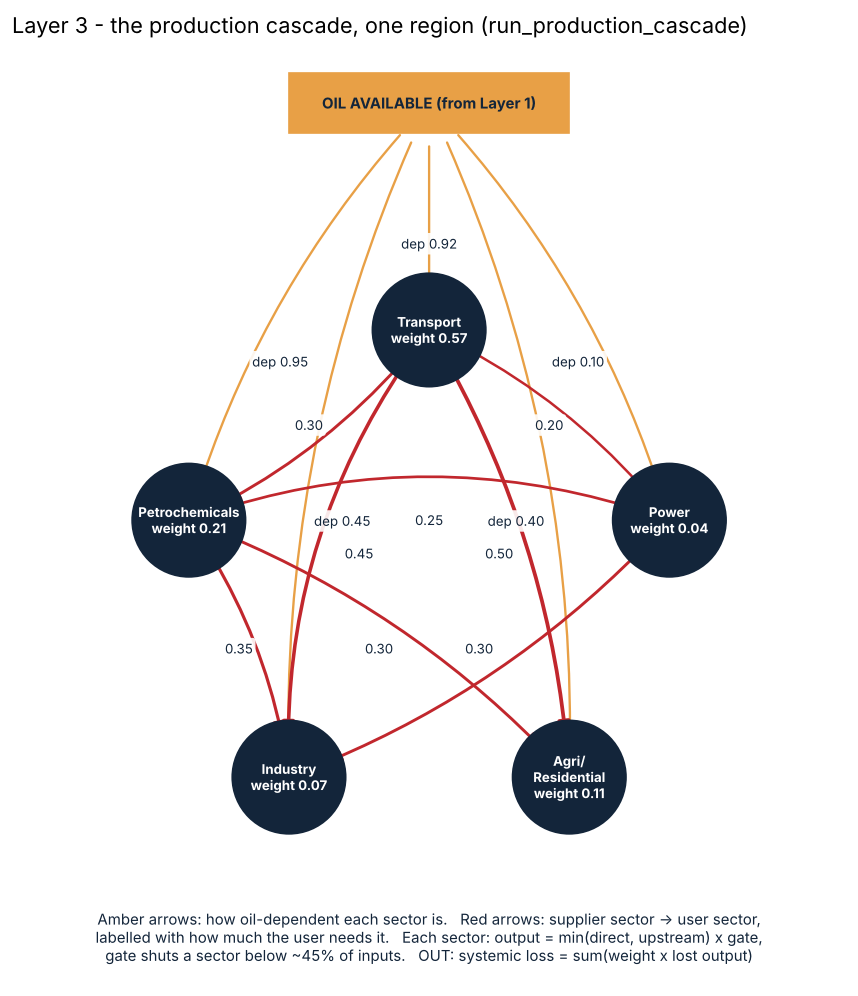
\includegraphics[width=0.49\textwidth]{figures/layer3_cascade.png}
\caption{Layers 2 and 3 as networks. Left: each region's demand responds to one world price with its own elasticity $e$; each strategic reserve (Mb; maximum draw, mb/d) supplies only its own region. Right: the five-sector cascade inside one region; amber arrows give oil dependence, red arrows supplier needs.}\label{fig:layers}
\end{figure}

\begin{figure}[H]
\centering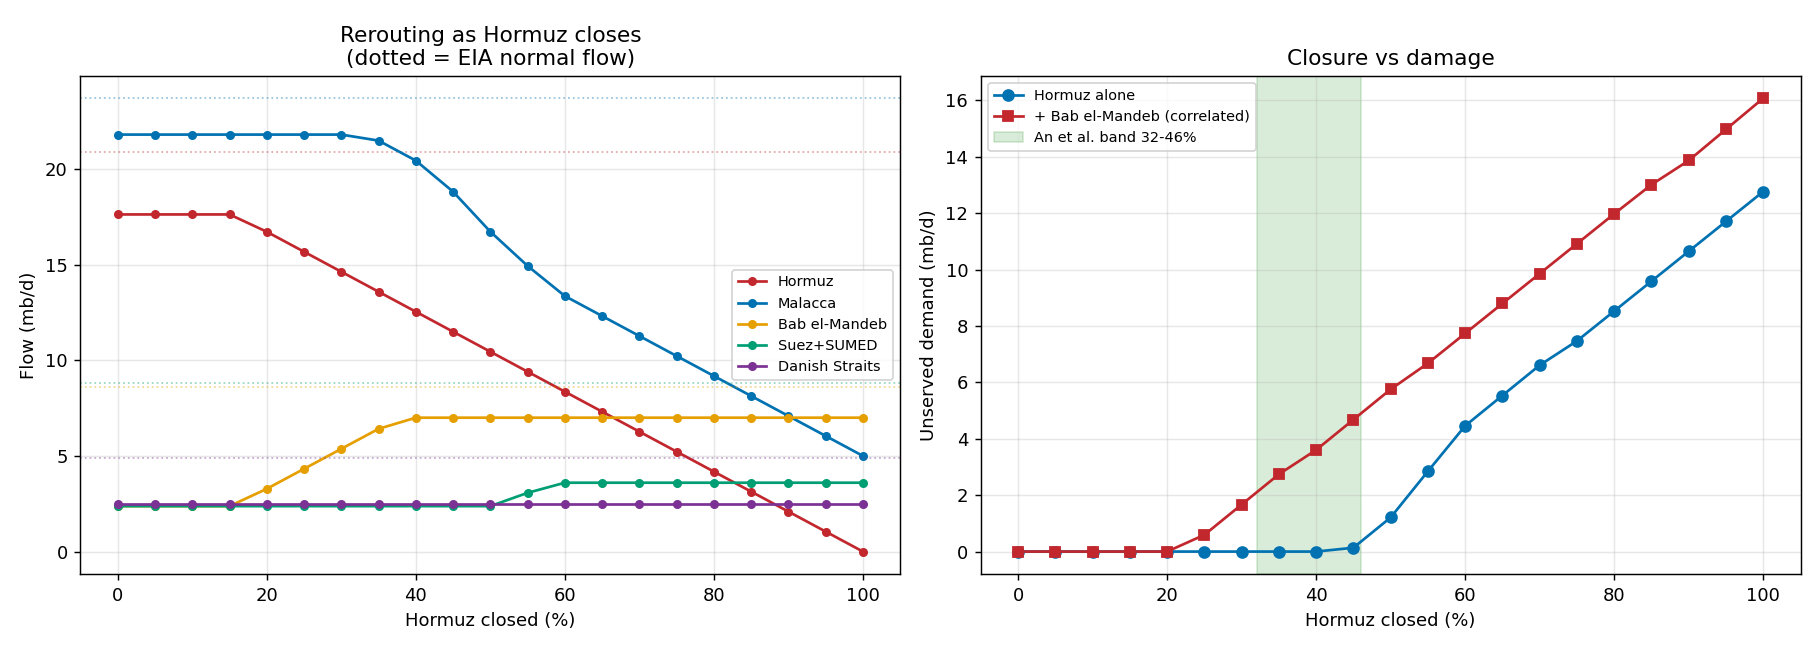
\includegraphics[width=1.00\textwidth]{figures/1_chokepoint_response.png}
\caption{Closure response. Left: chokepoint flows as Hormuz closes (dotted lines: EIA normal flows). Right: world unserved demand for Hormuz alone and with Bab el-Mandeb also closed; the shaded band is the 32--46\% threshold range of An et al. (2026), which uses a different failure definition.}\label{fig:closure}
\end{figure}

\begin{figure}[H]
\centering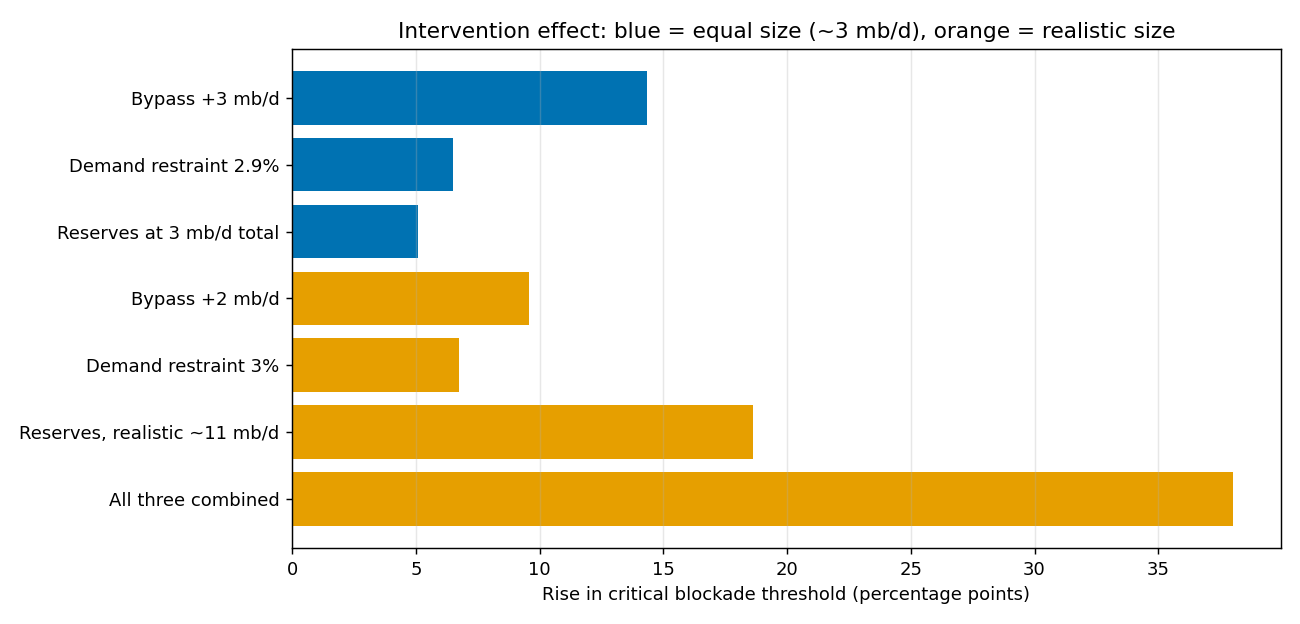
\includegraphics[width=0.83\textwidth]{figures/5_interventions_threshold.png}
\caption{Rise in the critical blockade intensity above the 53.1\% baseline (percentage points). Blue: interventions of equal size ($\sim$3\,mb/d each). Orange: realistic sizes. The realistic reserve effect lasts only until regional stocks run out.}\label{fig:interv}
\end{figure}

\begin{figure}[H]
\centering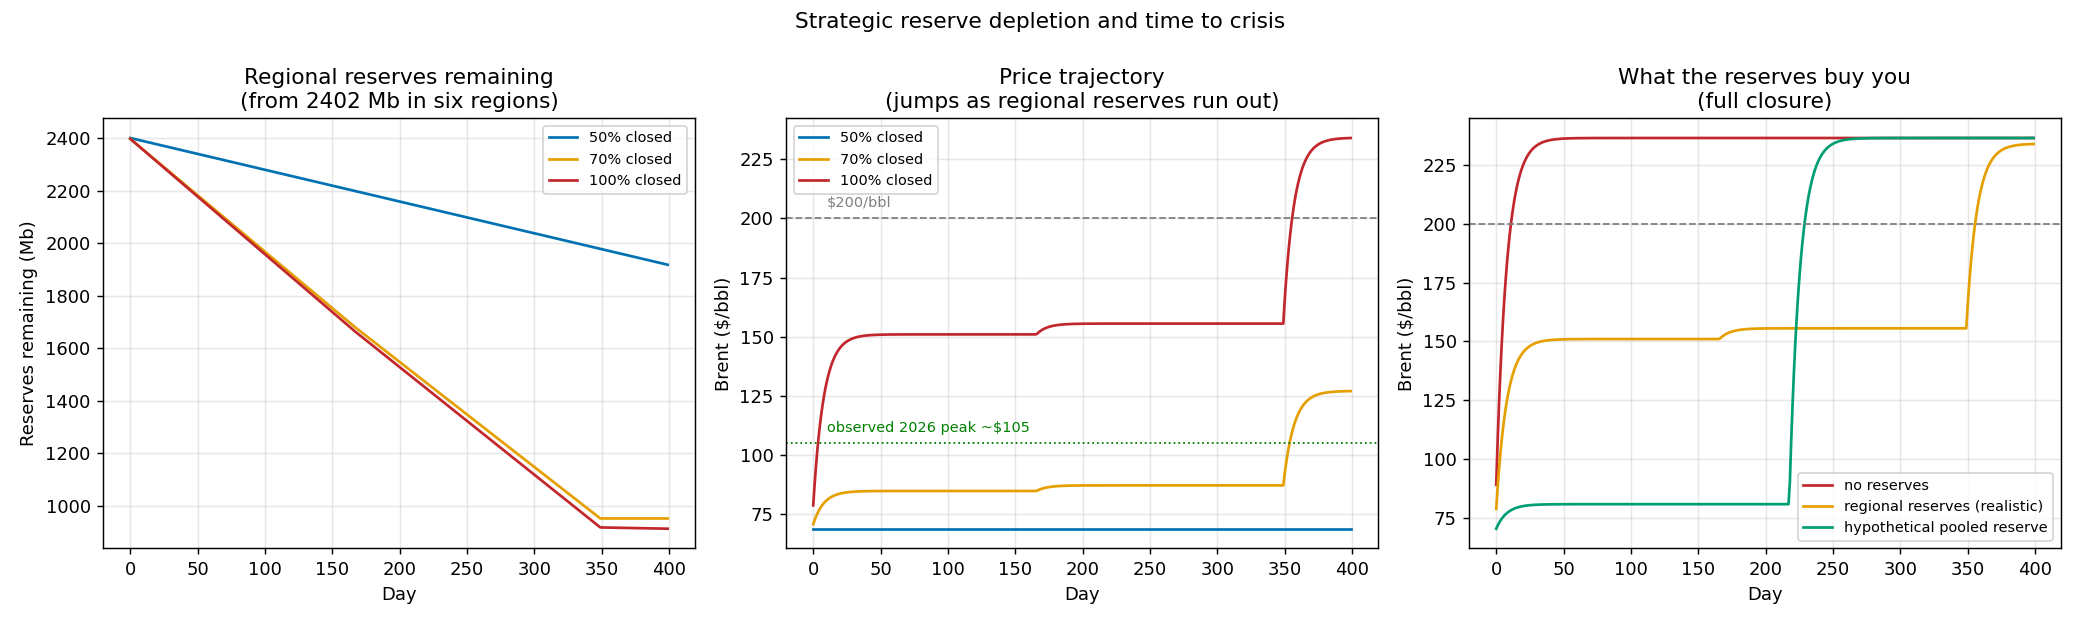
\includegraphics[width=1.00\textwidth]{figures/spr_depletion.png}
\caption{Strategic reserves. Left: total reserves remaining at three closure levels. Centre: Brent price path; steps occur as regional reserves run out (Other Asia on day 167, China on day 350). Right: full closure with no reserves, realistic regional reserves, and a hypothetical pooled reserve with the same total draw rate.}\label{fig:reserves}
\end{figure}

\begin{figure}[H]
\centering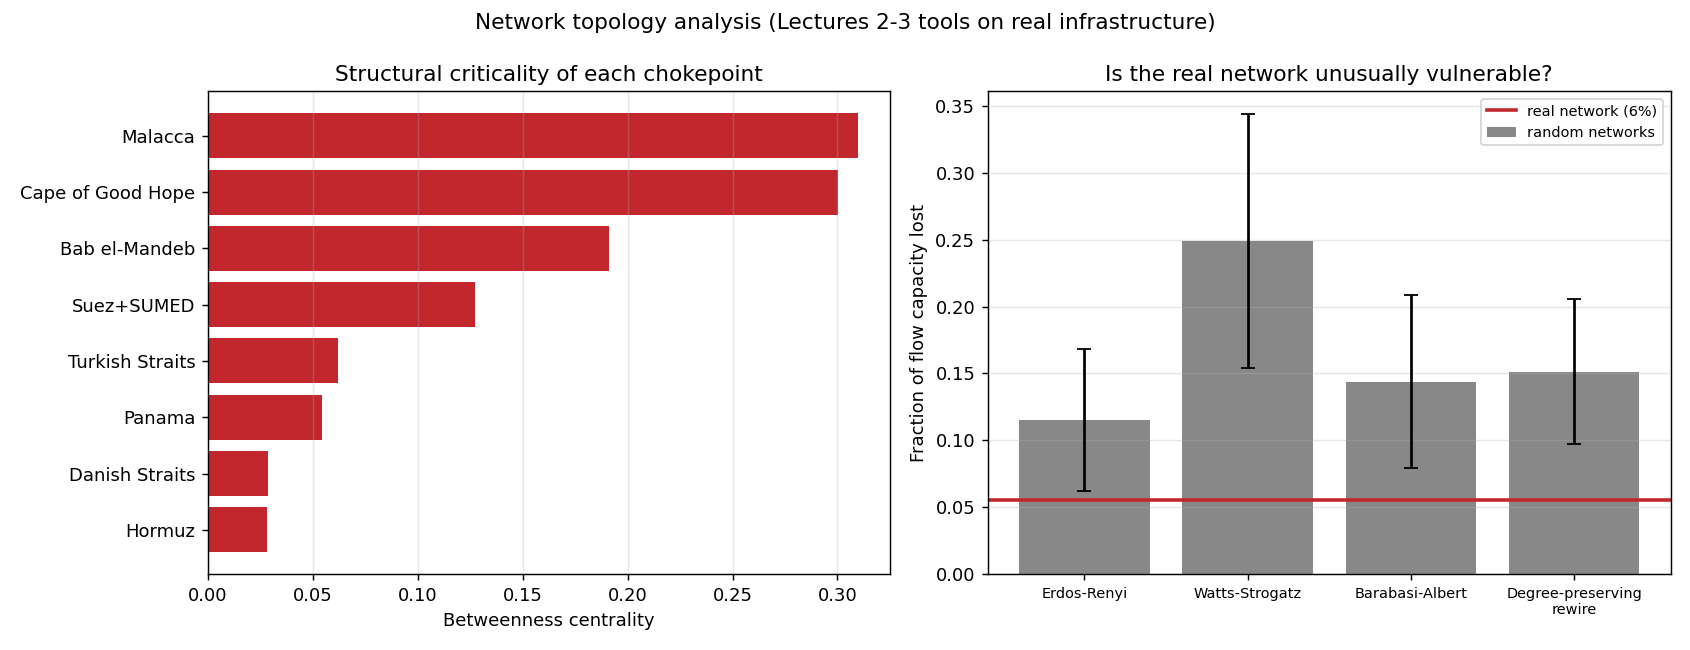
\includegraphics[width=0.96\textwidth]{figures/4_topology_comparison.png}
\caption{Topology. Left: betweenness centrality of each chokepoint. Right: share of flow capacity lost when the most central chokepoint is removed, for the real network (red line, 5.6\%) and 200 random graphs of each type with the same numbers of nodes and edges (mean $\pm$ one standard deviation).}\label{fig:topo}
\end{figure}

\begin{figure}[H]
\centering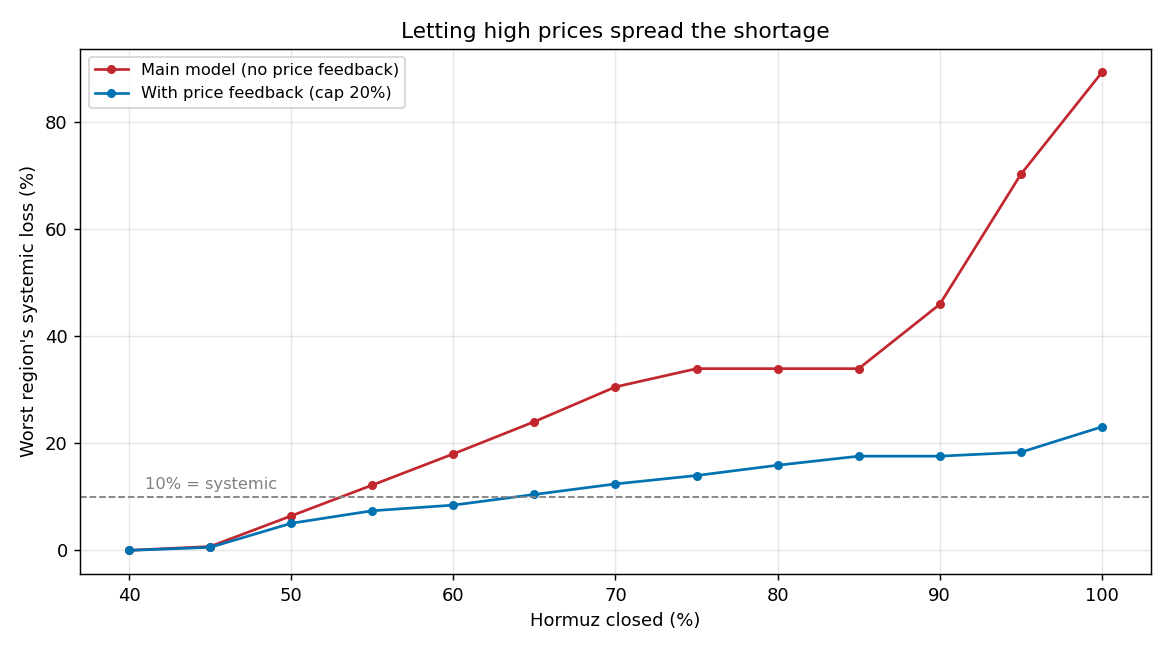
\includegraphics[width=0.73\textwidth]{figures/6_price_feedback.png}
\caption{Extension: worst-region systemic loss against Hormuz closure, main model and with price feedback (20\% cap). The dashed line marks the 10\% systemic criterion.}\label{fig:ext}
\end{figure}

\clearpage
\section*{Appendix A: Where each report criterion is addressed}

{\small
\renewcommand{\arraystretch}{1.15}
\begin{tabularx}{\textwidth}{@{}>{\raggedright\arraybackslash}p{4.2cm}>{\raggedright\arraybackslash}X@{}}
\toprule
\textbf{Rubric criterion} & \textbf{Where it is addressed} \\ \midrule
Background and research aims & Section~1: the 2026 closure and why it is a complex system; 2026 studies and network-science literature; research questions Q1--Q6. \\
Originality and contribution & Section~2 and Table~\ref{tab:lit}: model type, scale and scope compared with four 2026 studies; contributions (i)--(vi); taught models used only as null models. \\
Model specification and justification & Section~3: Table~\ref{tab:net} (nodes and edges), Figure~\ref{fig:flow} (how the layers connect), Equations~(1)--(6), data sources, assumptions and initial conditions (Section~3.6). \\
Experimental design & Section~4: one experiment per question, with parameter ranges, outcome measures, run lengths and repetition. \\
Results & Section~5 (one subsection per question, plus validation) and Figures~\ref{fig:map}--\ref{fig:ext}. \\
Discussion and conclusions & Section~6: interpretation of each question, comparison with An et al.\ (2026), limitations and future work. \\
Scientific writing and presentation & Five A4 pages of text (Sections 1--6), 11\,pt font, 1-inch margins; author--year citations; figures, references and appendices follow the text. \\
Links to simulations & Code, data and notebook: \url{https://github.com/raed-ra/cits4403-oil-chokepoint}. \\
\bottomrule
\end{tabularx}}

\section*{Appendix B: Use of generative AI}

Generative AI was used to assist with debugging and implementing the code and with drafting and editing this report. The research question, the modelling and data decisions and the review of the model's errors are the author's own, and every result reported has been checked against the code.

\end{document}
